    \documentclass[12pt,a4paper]{article}

    \usepackage[utf8]{inputenc}
    \usepackage[T1]{fontenc}
    \usepackage[brazil]{babel}
    \usepackage{geometry}
    \usepackage{graphicx}
    \usepackage{float}
    \usepackage{xcolor}
    \usepackage{hyperref}
    \usepackage{booktabs}
    \usepackage{longtable}
    \usepackage{listings}
    \usepackage{tikz}
    \usepackage{pdflscape}
    \usetikzlibrary{arrows.meta, positioning, shapes.geometric, shapes.symbols, fit, calc}

    \geometry{left=3cm,right=2cm,top=3cm,bottom=2cm}

    \hypersetup{
        colorlinks=true,
        linkcolor=blue,
        urlcolor=blue,
        citecolor=blue
    }

    \definecolor{codegray}{RGB}{245,245,245}
    \definecolor{codeborder}{RGB}{210,210,210}
    \definecolor{codecomment}{RGB}{90,120,90}
    \definecolor{codekeyword}{RGB}{0,70,140}
    \definecolor{codestring}{RGB}{150,60,40}

    \lstdefinestyle{cppstyle}{
        language=C++,
        basicstyle=\ttfamily\footnotesize,
        keywordstyle=\color{codekeyword}\bfseries,
        commentstyle=\color{codecomment},
        stringstyle=\color{codestring},
        backgroundcolor=\color{codegray},
        frame=single,
        rulecolor=\color{codeborder},
        numbers=left,
        numberstyle=\tiny,
        breaklines=true,
        tabsize=4,
        showstringspaces=false,
        captionpos=b,
        literate=
            {á}{{\'a}}1 {à}{{\`a}}1 {ã}{{\~a}}1 {â}{{\^a}}1
            {Á}{{\'A}}1 {À}{{\`A}}1 {Ã}{{\~A}}1 {Â}{{\^A}}1
            {é}{{\'e}}1 {ê}{{\^e}}1 {É}{{\'E}}1 {Ê}{{\^E}}1
            {í}{{\'i}}1 {Í}{{\'I}}1
            {ó}{{\'o}}1 {õ}{{\~o}}1 {ô}{{\^o}}1
            {Ó}{{\'O}}1 {Õ}{{\~O}}1 {Ô}{{\^O}}1
            {ú}{{\'u}}1 {Ú}{{\'U}}1
            {ç}{{\c{c}}}1 {Ç}{{\c{C}}}1
    }

    \lstdefinestyle{textstyle}{
        basicstyle=\ttfamily\footnotesize,
        backgroundcolor=\color{codegray},
        frame=single,
        rulecolor=\color{codeborder},
        numbers=none,
        breaklines=true,
        tabsize=4,
        showstringspaces=false,
        literate=
            {á}{{\'a}}1 {à}{{\`a}}1 {ã}{{\~a}}1 {â}{{\^a}}1
            {Á}{{\'A}}1 {À}{{\`A}}1 {Ã}{{\~A}}1 {Â}{{\^A}}1
            {é}{{\'e}}1 {ê}{{\^e}}1 {É}{{\'E}}1 {Ê}{{\^E}}1
            {í}{{\'i}}1 {Í}{{\'I}}1
            {ó}{{\'o}}1 {õ}{{\~o}}1 {ô}{{\^o}}1
            {Ó}{{\'O}}1 {Õ}{{\~O}}1 {Ô}{{\^O}}1
            {ú}{{\'u}}1 {Ú}{{\'U}}1
            {ç}{{\c{c}}}1 {Ç}{{\c{C}}}1
    }

    \newcommand{\FiguraTesteTerminal}[3]{
        \begin{figure}[H]
            \centering
            \IfFileExists{#1}{
                \includegraphics[width=\textwidth,height=0.32\textheight,keepaspectratio]{#1}
            }{
                \fbox{\parbox{0.9\textwidth}{Arquivo de print nao encontrado: \texttt{\detokenize{#1}}}}
            }
            \caption{#2}
            \label{#3}
        \end{figure}
    }

    \title{Sistema de Inspeção Automática de Túneis\\Relatório da Etapa 1}
    \author{
        Nome do Integrante Leandro Lopo -- Matrícula 2021020520\\
        Nome do Integrante Rodrigo Martins-- Matrícula 000000\\
    }
    \date{Automação em Tempo Real -- 2026/1}

    \begin{document}

    \pagenumbering{gobble}
    \begin{titlepage}
        \centering
        \vspace*{2cm}
        {\Large Universidade Federal de Minas Gerais\par}
        \vspace{0.5cm}
        {\large Automação em Tempo Real\par}
        \vspace{2cm}
        {\Huge\bfseries Sistema de Inspeção Automática de Túneis\par}
        \vspace{0.5cm}
        {\Large Relatório da Etapa 1\par}
        \vspace{2cm}

        \begin{tabular}{ll}
            Leandro Lopo -- Matrícula 2021020520 \\
            Rodrigo Martins -- Matrícula 2023421459 \\
        \end{tabular}

        \vfill
        Professor: Leandro Freitas\par
        \vspace{0.5cm}
        Belo Horizonte\par
        \today
    \end{titlepage}

    \pagenumbering{roman}
    \tableofcontents
    \newpage
    \pagenumbering{arabic}

    \section{Introdução}

    Este trabalho desenvolve a arquitetura inicial de um sistema de inspeção automática de túneis. O robô se desloca horizontalmente, mede a distância até o teto com um LIDAR, reconstrói o perfil da superfície e detecta variações bruscas que indicam possíveis buracos ou saliências.

    Na Etapa 1, o objetivo é definir a arquitetura completa do projeto e implementar o núcleo interno do robô em C++. Essa implementação inclui threads, buffers compartilhados, mutexes, variáveis de condição e testes preliminares para verificar se as tarefas trocam dados de forma coerente.

    \begin{figure}[H]
        \centering
        \begin{tikzpicture}[
            scale=0.95,
            tunnel/.style={draw, thick, rounded corners=2pt},
            robot/.style={draw, thick, fill=gray!20, minimum width=1.6cm, minimum height=0.6cm},
            sensor/.style={->, thick, green!60!black},
            alert/.style={draw, thick, fill=red!15, rounded corners=2pt, align=center},
            axis/.style={->, thick}
        ]
            \draw[tunnel, fill=brown!10] (0,0) -- (0,4) -- (2.2,4) .. controls (2.5,3.2) and (3.2,3.2) .. (3.5,4) -- (6.2,4) .. controls (6.5,4.7) and (7.4,4.7) .. (7.7,4) -- (10,4) -- (10,0) -- cycle;
            \draw[thick] (0,0) -- (10,0);

            \node[robot] (r) at (5,0.45) {Robô};
            \draw[sensor] (5,0.8) -- (5,4.0) node[midway,right] {LIDAR};
            \draw[axis] (0.8,-0.5) -- (9.3,-0.5) node[right] {$x$};
            \draw[axis] (0.8,-0.5) -- (0.8,4.4) node[above] {$y$};

            \node[alert] at (2.9,4.6) {Buraco\\detectado};
            \node[alert] at (7.0,5.2) {Saliência\\detectada};

            \draw[blue, thick] (1.2,-1.2) -- (2.4,-1.2) -- (2.7,-1.8) -- (3.2,-1.8) -- (3.5,-1.2) -- (6.0,-1.2) -- (6.4,-0.7) -- (7.3,-0.7) -- (7.7,-1.2) -- (9.0,-1.2);
            \node at (5,-2.1) {Perfil reconstruído do teto a partir das medições};
        \end{tikzpicture}
        \caption{Ilustração própria do problema tratado: robô inspecionando o teto de um túnel em vista lateral 2D.}
        \label{fig:introducao}
    \end{figure}

    \section{Proposta de Arquitetura}

    A arquitetura proposta cobre o projeto completo, e não apenas o subconjunto implementado nesta primeira entrega. O sistema foi dividido em dois níveis: um núcleo embarcado em C++, responsável pelas tarefas de tempo real do robô, e processos externos para simulação, operação remota e comunicação publisher/subscriber. Essa separação acompanha a organização indicada no enunciado e deixa claro quais partes pertencem ao controle interno do robô e quais partes serão integradas por IPC na etapa seguinte.

    No núcleo do robô, as tarefas internas foram modeladas como threads C++ dentro de um único processo. A comunicação entre essas threads ocorre por memória compartilhada, com buffers protegidos por \texttt{std::mutex} e \texttt{std::condition\_variable}. Essa decisão é adequada para a Etapa 1 porque permite demonstrar diretamente os conceitos de concorrência, região crítica, produtor-consumidor e sincronização.

    Os processos externos de simulação, operação remota e broker MQTT foram especificados na arquitetura completa, mas não implementados nesta etapa. Na Etapa 1, a thread \texttt{SimulacaoSensores} substitui temporariamente a interface de simulação para alimentar os buffers internos e permitir testes preliminares. Na Etapa 2, essa thread de teste deve ser removida ou substituída pela entrada de dados recebida via MQTT.

    \subsection{Diagrama da Arquitetura}

    \begin{figure}[H]
        \centering
        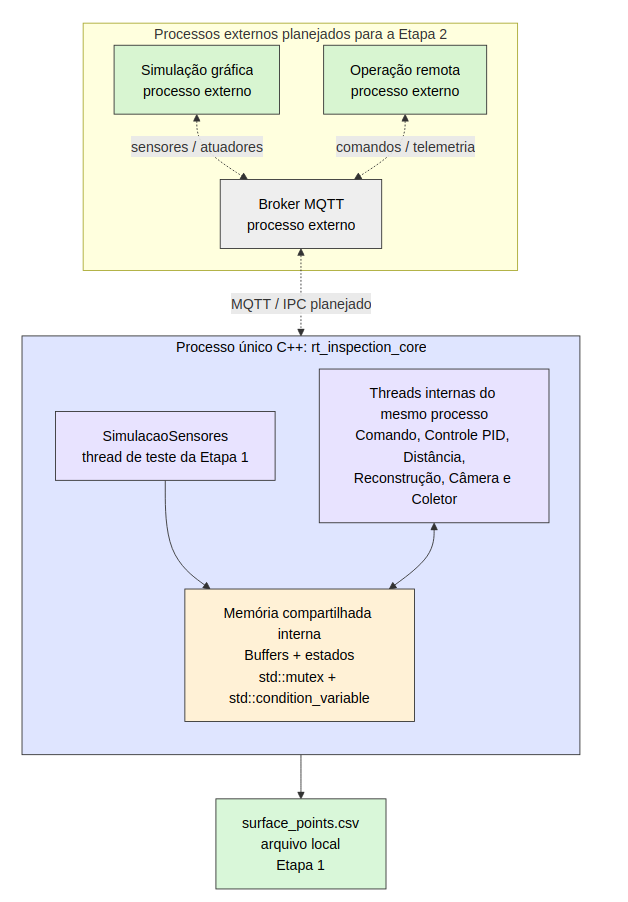
\includegraphics[width=0.82\textwidth,height=0.68\textheight,keepaspectratio]{figuras/arquitetura_completa.png}
        \caption{Diagrama de contêineres da arquitetura completa.}
        \label{fig:arquitetura-completa}
    \end{figure}

    A Figura~\ref{fig:arquitetura-completa} usa uma visão de contêineres, semelhante ao modelo C4 usado em documentação de sistemas. Ela separa processos externos, broker MQTT, núcleo C++ e armazenamento local. No diagrama, as setas tracejadas representam interfaces MQTT planejadas para a Etapa 2, enquanto as setas contínuas representam fluxos internos ou saída local do núcleo C++ na Etapa 1. O detalhamento interno do núcleo é apresentado na Figura~\ref{fig:arquitetura}.

    \subsection{Interações Planejadas Entre Processos}

    As interações externas do projeto completo serão implementadas por MQTT na Etapa 2. O broker atua como intermediário entre processos, seguindo o modelo publisher/subscriber. A Tabela~\ref{tab:mqtt} resume os fluxos planejados.

    \begin{longtable}{p{3.5cm}p{3.5cm}p{3.5cm}p{3.5cm}}
    \caption{Comunicação planejada entre processos externos e núcleo do robô.}
    \label{tab:mqtt}\\
    \toprule
    \textbf{Origem} & \textbf{Destino} & \textbf{Mecanismo} & \textbf{Dados} \\
    \midrule
    \endhead
    Simulação gráfica & Núcleo C++ & MQTT: \texttt{sim/sensors} & Leituras de LIDAR e encoder. \\
    Núcleo C++ & Simulação gráfica & MQTT: \texttt{core/actuators} & Aceleração e comando de câmera. \\
    Operação remota & Núcleo C++ & MQTT: \texttt{remote/commands} & Modo manual/automático e setpoints. \\
    Núcleo C++ & Operação remota & MQTT: \texttt{core/state} & Posição, velocidade e estado de inspeção. \\
    Núcleo C++ & Operação remota & MQTT: \texttt{core/surface} & Pontos reconstruídos e confiança. \\
    \bottomrule
    \end{longtable}

    \begin{figure}[H]
        \centering
        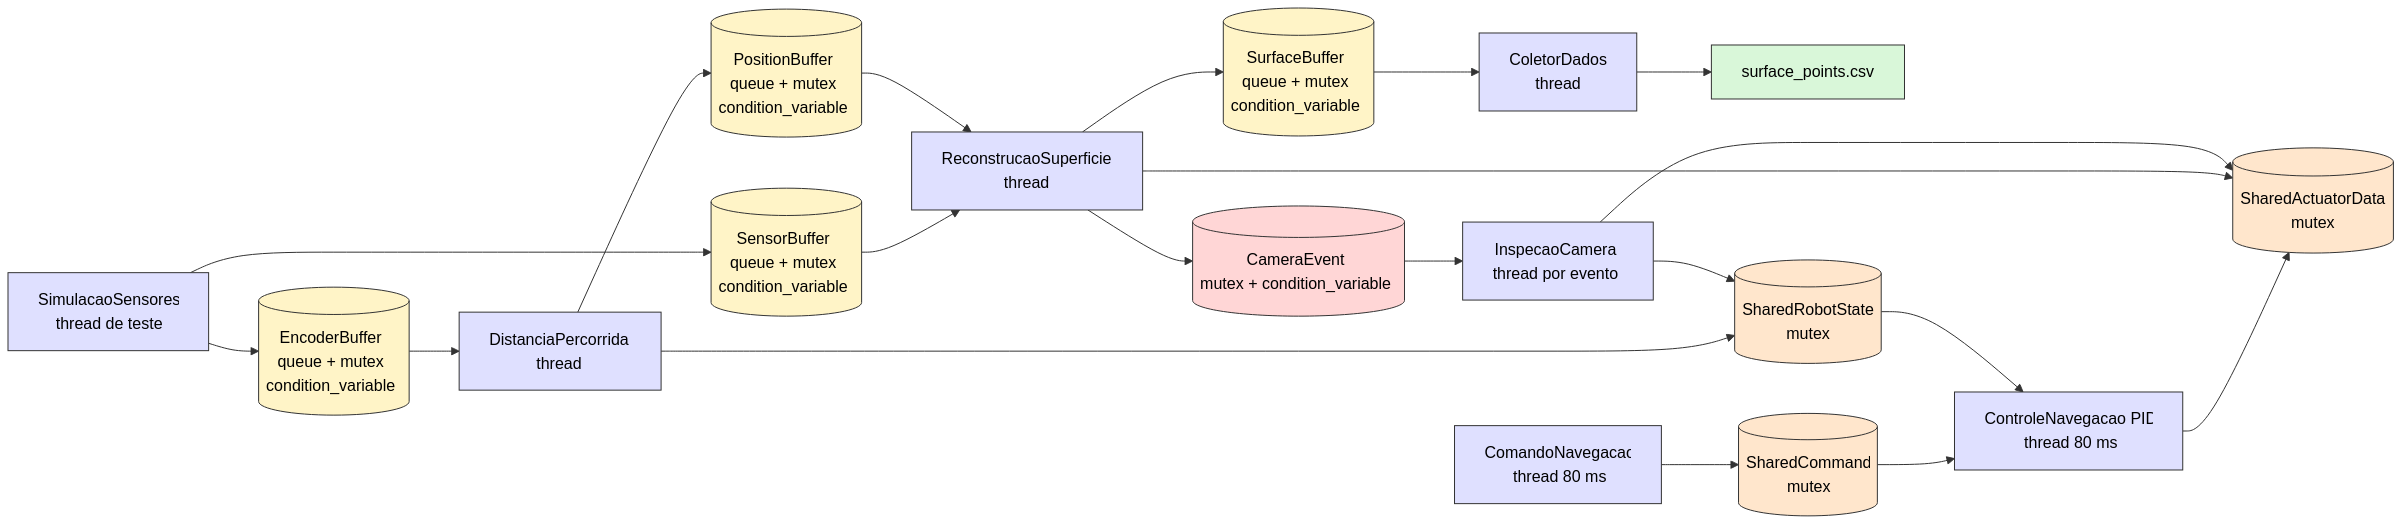
\includegraphics[width=\textwidth,height=0.30\textheight,keepaspectratio]{figuras/nucleo_cpp_fluxo.png}
        \caption{Diagrama de componentes e fluxo de dados do núcleo C++ implementado na Etapa 1.}
        \label{fig:arquitetura}
    \end{figure}

    \subsection{Tarefas Implementadas}

    \begin{longtable}{p{4.8cm}p{3.3cm}p{5.9cm}}
    \toprule
    \textbf{Tarefa} & \textbf{Tipo} & \textbf{Responsabilidade} \\
    \midrule
    \endhead
    \texttt{SimulacaoSensores} & Thread C++ de teste & Gera dados simulados de LIDAR e encoder para testar os buffers da Etapa 1. \\
    \texttt{ReconstrucaoSuperficie} & Thread C++ & Consome leituras de LIDAR e posições calculadas, aplica média móvel, gera pontos de superfície e detecta anomalias. \\
    \texttt{DistanciaPercorrida} & Thread C++ & Consome o encoder, calcula a posição horizontal do robô e publica amostras de posição. \\
    \texttt{ColetorDados} & Thread C++ & Consome pontos reconstruídos, calcula confiança online e grava os dados em CSV. \\
    \texttt{ComandoNavegacao} & Thread C++ cíclica & Simula comando de operação remota na Etapa 1, configurando modo automático e setpoint. \\
    \texttt{ControleNavegacao} & Thread C++ cíclica & Aplica controle PID simples e gera aceleração. \\
    \texttt{InspecaoCamera} & Thread C++ por evento & Aguarda sinal de falha e executa processamento pesado usando CPU. \\
    \bottomrule
    \end{longtable}

    \subsection{Buffers e Estados Compartilhados}

    Os buffers implementam o padrão produtor-consumidor. Cada buffer possui uma fila, um mutex, uma variável de condição e uma flag de finalização.

    \begin{longtable}{p{3.5cm}p{5.3cm}p{5.4cm}}
    \toprule
    \textbf{Estrutura} & \textbf{Fluxo} & \textbf{Sincronização} \\
    \midrule
    \endhead
    \texttt{SensorBuffer} & \texttt{SimulacaoSensores} $\rightarrow$ \texttt{ReconstrucaoSuperficie} & \texttt{mutex\_sensor} e \texttt{dado\_disponivel\_var}. \\
    \texttt{EncoderBuffer} & \texttt{SimulacaoSensores} $\rightarrow$ \texttt{DistanciaPercorrida} & \texttt{mutex\_encoder} e \texttt{encoder\_disponivel\_var}. \\
    \texttt{PositionBuffer} & \texttt{DistanciaPercorrida} $\rightarrow$ \texttt{ReconstrucaoSuperficie} & \texttt{mutex\_posicao} e \texttt{posicao\_disponivel\_var}. \\
    \texttt{SurfaceBuffer} & \texttt{ReconstrucaoSuperficie} $\rightarrow$ \texttt{ColetorDados} & \texttt{mutex\_superficie} e \texttt{surface\_point\_var}. \\
    \texttt{CameraEvent} & \texttt{ReconstrucaoSuperficie} $\rightarrow$ \texttt{InspecaoCamera} & \texttt{mutex\_camera} e \texttt{camera\_event\_var}. \\
    \bottomrule
    \end{longtable}

    Além dos buffers, foram utilizados estados compartilhados protegidos por mutex:

    \begin{itemize}
        \item \texttt{SharedRobotState}: armazena posição, velocidade, modo automático e estado de inspeção.
        \item \texttt{SharedCommand}: armazena comandos simulados para a Etapa 1.
        \item \texttt{SharedActuatorData}: armazena aceleração e comando de câmera.
        \item \texttt{SharedSystemControl}: controla o encerramento das tarefas cíclicas.
    \end{itemize}

    \subsection{Mecanismos de Sincronização}

    O \texttt{std::mutex} é usado para proteger regiões críticas, como inserção e remoção de dados em filas ou leitura e escrita em estados compartilhados. A regra usada no código foi manter o mutex travado apenas durante o acesso ao dado compartilhado, copiando o valor para uma variável local e realizando o processamento fora da região crítica.

    A \texttt{std::condition\_variable} é usada para evitar espera ocupada. As tarefas consumidoras ficam bloqueadas até que uma tarefa produtora insira um novo dado no buffer e chame \texttt{notify\_one()}. Essa estratégia reduz uso desnecessário de CPU e evita laços de polling.

    \section{Implementação Desenvolvida}

    Esta seção apresenta os principais trechos de código do sistema e a justificativa das decisões tomadas em cada parte da implementação. Os trechos foram escolhidos por representarem os mecanismos centrais do trabalho: definição dos dados, comunicação por buffers, sincronização, reconstrução da superfície, detecção de falhas, controle de navegação e acionamento da câmera.

    \subsection{Tipos de Dados}

    O primeiro passo da implementação foi definir estruturas simples para representar as mensagens trocadas entre as tarefas. Essa escolha evita passar vários parâmetros soltos entre threads e deixa explícito qual informação circula em cada buffer. \texttt{SensorData} representa a leitura combinada de LIDAR e encoder, \texttt{EncoderData} separa o fluxo usado pela tarefa de distância, \texttt{PositionData} carrega a posição calculada a partir do encoder, e \texttt{SurfacePoint} representa o ponto reconstruído do teto.

    \begin{figure}[H]
        \centering
        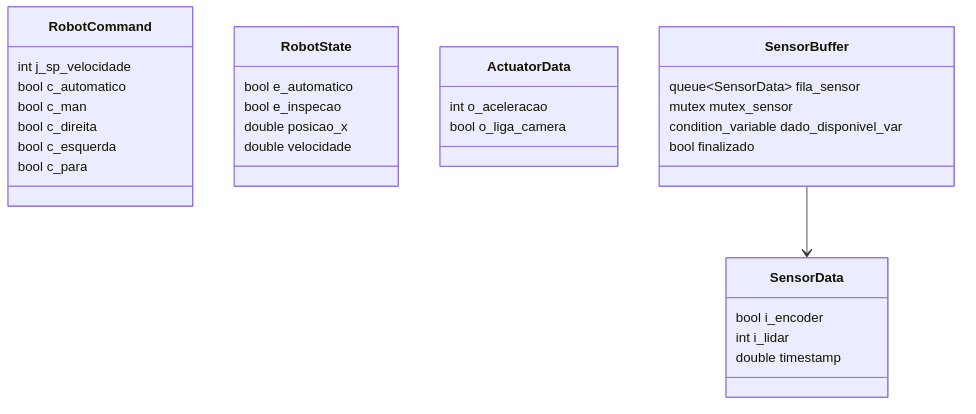
\includegraphics[width=\textwidth,height=0.25\textheight,keepaspectratio]{figuras/estruturas_dados_uml_2.png}
        \caption{Diagrama UML simplificado das estruturas de comando, estado, atuadores e buffers de sensores.}
        \label{fig:uml-dados}
    \end{figure}

    \begin{figure}[H]
        \centering
        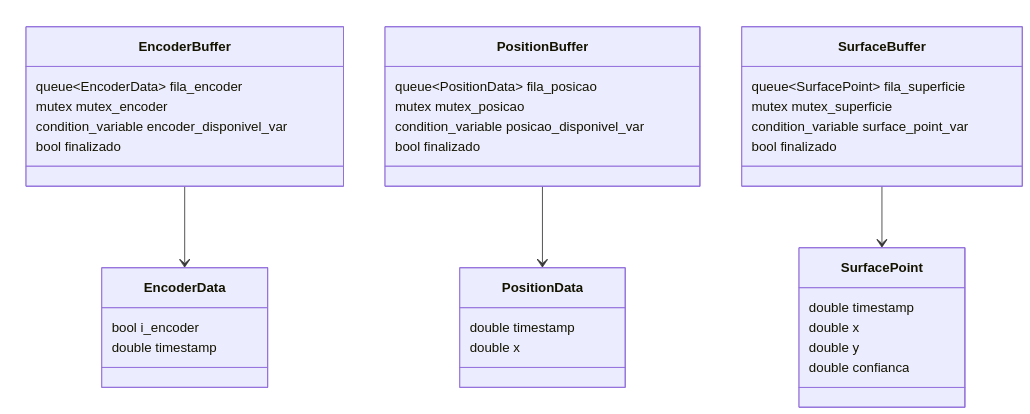
\includegraphics[width=\textwidth,height=0.25\textheight,keepaspectratio]{figuras/estruturas_dados_uml_1.png}
        \caption{Diagrama UML simplificado dos buffers de posição e superfície e das mensagens associadas.}
        \label{fig:uml-dados-parte-2}
    \end{figure}

    As Figuras~\ref{fig:uml-dados} e~\ref{fig:uml-dados-parte-2} resumem a relação entre as estruturas usadas no código. Os trechos seguintes mostram as definições essenciais que sustentam a troca de dados entre as tarefas.

    \begin{lstlisting}[style=cppstyle]
    struct SensorData {
        bool i_encoder;
        int i_lidar;
        double timestamp;
    };

    struct EncoderData {
        bool i_encoder;
        double timestamp;
    };

    struct PositionData {
        double timestamp;
        double x;
    };

    struct SurfacePoint {
        double timestamp;
        double x;
        double y;
        double confianca;
    };
    \end{lstlisting}

    Separar \texttt{EncoderData} de \texttt{SensorData} foi importante para evitar que duas tarefas consumidoras retirassem dados da mesma fila. A reconstrução consome o fluxo de sensores e também recebe a posição calculada pela tarefa de distância através de \texttt{PositionBuffer}. Isso evita que a coordenada horizontal de um ponto reconstruído dependa do instante de escalonamento de outra thread.

    \subsection{Buffers Sincronizados}

    Os buffers foram implementados seguindo o padrão produtor-consumidor. Cada buffer possui uma fila, um mutex, uma variável de condição e uma flag de finalização. Essa estrutura foi escolhida porque permite que uma tarefa produza dados em seu próprio ritmo e outra tarefa consuma esses dados sem espera ocupada.

    \begin{lstlisting}[style=cppstyle]
    struct SensorBuffer {
        std::queue<SensorData> fila_sensor;
        std::mutex mutex_sensor;
        std::condition_variable dado_disponivel_var;
        bool finalizado = false;
    };

    struct SurfaceBuffer {
        std::queue<SurfacePoint> fila_superficie;
        std::mutex mutex_superficie;
        std::condition_variable surface_point_var;
        bool finalizado = false;
    };

    struct PositionBuffer {
        std::queue<PositionData> fila_posicao;
        std::mutex mutex_posicao;
        std::condition_variable posicao_disponivel_var;
        bool finalizado = false;
    };
    \end{lstlisting}

    O \texttt{mutex} protege o acesso à fila. A \texttt{condition\_variable} permite que a tarefa consumidora durma enquanto não há dados disponíveis. A flag \texttt{finalizado} evita que a consumidora fique bloqueada indefinidamente ao final da simulação.

    \subsection{Simulação dos Sensores}

    A tarefa de simulação foi usada na Etapa 1 para substituir temporariamente a interface gráfica de simulação que será implementada na Etapa 2. Ela gera leituras falsas, alterna o encoder e injeta uma anomalia no LIDAR para testar a detecção de falhas.

    \begin{lstlisting}[style=cppstyle]
    for (int i = 0; i < 10; i++) {
        estado_encoder = !estado_encoder;

        SensorData leitura;
        leitura.i_encoder = estado_encoder;
        leitura.i_lidar = (i == 5) ? 140 : 100 + i;
        leitura.timestamp = TempoAtualSegundos();

        EncoderData encoder{leitura.i_encoder, leitura.timestamp};

        {
            std::lock_guard<std::mutex> trava(encoderBuffer.mutex_encoder);
            encoderBuffer.fila_encoder.push(encoder);
        }
        encoderBuffer.encoder_disponivel_var.notify_one();

        {
            std::lock_guard<std::mutex> trava(sensorBuffer.mutex_sensor);
            sensorBuffer.fila_sensor.push(leitura);
        }
        sensorBuffer.dado_disponivel_var.notify_one();

        std::this_thread::sleep_for(std::chrono::milliseconds(500));
    }
    \end{lstlisting}

    A leitura anômala \texttt{i\_lidar = 140} foi colocada para simular uma variação brusca no teto. O uso de \texttt{sleep\_for} aqui representa o intervalo entre leituras de sensores simulados. Isso é diferente da tarefa de câmera, que não deve ser simulada apenas com \texttt{sleep}, pois o enunciado exige processamento pesado.

    \subsection{Consumo com Variável de Condição}

    As tarefas consumidoras usam \texttt{condition\_variable} para aguardar dados. Essa decisão evita que a thread execute um laço verificando a fila repetidamente, o que desperdiçaria CPU.

    \begin{lstlisting}[style=cppstyle]
    SensorData leitura;

    {
        std::unique_lock<std::mutex> trava(buffer.mutex_sensor);

        buffer.dado_disponivel_var.wait(trava, [&buffer] {
            return !buffer.fila_sensor.empty() || buffer.finalizado;
        });

        if (buffer.fila_sensor.empty() && buffer.finalizado) {
            break;
        }

        leitura = buffer.fila_sensor.front();
        buffer.fila_sensor.pop();
    }
    \end{lstlisting}

    O processamento é feito fora da região crítica. Assim, o mutex fica travado apenas pelo tempo necessário para retirar o dado da fila, reduzindo contenção entre threads.

    \subsection{Reconstrução da Superfície}

    A reconstrução aplica uma média móvel de três amostras no LIDAR. Essa técnica foi escolhida por ser simples, online e suficiente para reduzir ruídos iniciais sem exigir armazenamento de todo o histórico.

    \begin{lstlisting}[style=cppstyle]
    ultimasLeituras.push(leitura.i_lidar);
    somaLeituras += leitura.i_lidar;

    if (ultimasLeituras.size() > tamanhoJanela) {
        somaLeituras -= ultimasLeituras.front();
        ultimasLeituras.pop();
    }

    double media_movel =
        static_cast<double>(somaLeituras) / ultimasLeituras.size();

    SurfacePoint ponto;
    ponto.timestamp = leitura.timestamp;
    ponto.x = posicao.x;
    ponto.y = media_movel;
    ponto.confianca = 1.0;
    \end{lstlisting}

    A coordenada \texttt{x} vem do \texttt{PositionBuffer}, produzido pela tarefa de distância percorrida. Dessa forma, cada ponto reconstruído combina a leitura vertical filtrada com a posição horizontal correspondente à mesma amostra de sensor.

    \subsection{Detecção de Falha}

    A falha é detectada comparando a média móvel atual com a média anterior. A regra foi escolhida por ser simples de testar e por representar a ideia central do problema: buracos e saliências aparecem como variações bruscas no perfil do teto.

    \begin{lstlisting}[style=cppstyle]
    const double variacao = std::abs(media_movel - mediaAnterior);

    if (variacao > limiteFalha && !falhaJaDetectada) {
        falhaJaDetectada = true;

        {
            std::lock_guard<std::mutex> trava(robotState.mutex_estado);
            robotState.estado.e_inspecao = true;
        }

        {
            std::lock_guard<std::mutex> trava(sharedActuatorData.mutex_atuadores);
            sharedActuatorData.atuadores.o_liga_camera = true;
        }

        {
            std::lock_guard<std::mutex> trava(cameraEvent.mutex_camera);
            cameraEvent.falha_detectada = true;
            cameraEvent.timestamp = ponto.timestamp;
            cameraEvent.x = ponto.x;
            cameraEvent.y = ponto.y;
        }

        cameraEvent.camera_event_var.notify_one();
    }
    \end{lstlisting}

    Quando a falha é encontrada, a reconstrução atualiza o estado do robô, liga a câmera e sinaliza o evento que acorda a tarefa \texttt{InspecaoCamera}. A flag \texttt{falhaJaDetectada} evita múltiplos disparos para a mesma anomalia simulada.

    \subsection{Distância Percorrida}

    A tarefa \texttt{DistanciaPercorrida} implementa a regra do enunciado: o encoder troca de estado a cada metro percorrido. Sempre que o valor atual do encoder difere do anterior, a posição horizontal é incrementada. Além de atualizar \texttt{SharedRobotState}, a tarefa publica a posição em \texttt{PositionBuffer}, permitindo que a reconstrução receba uma posição coerente com cada leitura de LIDAR.

    \begin{lstlisting}[style=cppstyle]
    bool houveMudanca = leitura.i_encoder != encoderAnterior;

    if (leitura.i_encoder != encoderAnterior) {
        encoderAnterior = leitura.i_encoder;
    }

    PositionData posicao;
    posicao.timestamp = leitura.timestamp;

    {
        std::lock_guard<std::mutex> trava(robotState.mutex_estado);

        if (houveMudanca) {
            robotState.estado.posicao_x += 1.0;
        }

        posicao.x = robotState.estado.posicao_x;
    }

    {
        std::lock_guard<std::mutex> trava(positionBuffer.mutex_posicao);
        positionBuffer.fila_posicao.push(posicao);
    }
    positionBuffer.posicao_disponivel_var.notify_one();
    \end{lstlisting}

    O estado do robô foi centralizado em \texttt{SharedRobotState} para que a posição também possa ser usada por outras tarefas. O \texttt{PositionBuffer} foi adicionado especificamente para manter a ordem temporal entre a leitura do sensor e a posição usada na reconstrução.

    \subsection{Coletor de Dados}

    O coletor recebe os pontos reconstruídos e grava o arquivo CSV. Além disso, calcula uma confiança simples com base na quantidade de pontos próximos já observados. Essa escolha atende ao requisito de análise online, mantendo a implementação simples para a Etapa 1.

    \begin{lstlisting}[style=cppstyle]
    int pontosProximos = 1;

    for (const SurfacePoint &anterior : historico) {
        const bool proximoEmX = std::abs(anterior.x - ponto.x) <= 2.0;
        const bool proximoEmY = std::abs(anterior.y - ponto.y) <= 15.0;

        if (proximoEmX && proximoEmY) {
            pontosProximos++;
        }
    }

    ponto.confianca = std::min(1.0, pontosProximos / 5.0);
    historico.push_back(ponto);

    arquivo << ponto.timestamp << ","
            << ponto.x << ","
            << ponto.y << ","
            << ponto.confianca << "\n";
    \end{lstlisting}

    O CSV permite verificar o perfil reconstruído e serve como evidência objetiva dos testes realizados.

    \subsection{Controle de Navegação}

    O controle de navegação foi implementado como um PID simples. Essa escolha aproxima a implementação do comportamento esperado para uma malha de controle real, sem esconder a lógica principal em bibliotecas externas. O controlador lê o setpoint produzido pela tarefa \texttt{ComandoNavegacao}, compara com a velocidade atual armazenada em \texttt{SharedRobotState} e escreve a aceleração em \texttt{SharedActuatorData}.

    \begin{lstlisting}[style=cppstyle]
    const double kp = 25.0;
    const double ki = 1.5;
    const double kd = 4.0;
    const double periodoSegundos = 0.08;
    const double limiteIntegral = 20.0;

    const double setpointVelocidade =
        emInspecao ? std::min(static_cast<double>(comando.j_sp_velocidade), 1.0)
                : static_cast<double>(comando.j_sp_velocidade);

    const double erro = setpointVelocidade - velocidadeAtual;
    integralErro = std::clamp(integralErro + erro * periodoSegundos,
                            -limiteIntegral, limiteIntegral);
    const double derivadaErro = (erro - erroAnterior) / periodoSegundos;
    erroAnterior = erro;

    const double saidaPid = kp * erro + ki * integralErro + kd * derivadaErro;
    const int aceleracao = static_cast<int>(
        std::clamp(saidaPid, -100.0, 100.0));

    {
        std::lock_guard<std::mutex> trava(sharedActuatorData.mutex_atuadores);
        sharedActuatorData.atuadores.o_aceleracao = aceleracao;
        sharedActuatorData.atuadores.o_liga_camera = emInspecao;
    }
    \end{lstlisting}

    Os ganhos foram mantidos conservadores para evitar oscilações grandes na simulação preliminar. O termo integral é limitado para evitar acúmulo excessivo de erro, e a saída do controlador é saturada no intervalo de aceleração permitido. Quando o robô entra em inspeção, o setpoint é limitado para reduzir a velocidade. Essa decisão acompanha o comportamento pedido no enunciado: ao detectar falha, o robô deve navegar mais devagar e acionar a câmera.

    \subsection{Inspeção por Câmera}

    A tarefa de câmera é acionada por evento. Ao acordar, ela executa um laço computacional com funções matemáticas, simulando processamento pesado de imagem. Essa escolha foi feita porque o enunciado especifica que essa tarefa deve usar o processador e não apenas dormir.

    \begin{lstlisting}[style=cppstyle]
    cameraEvent.camera_event_var.wait(trava, [&cameraEvent] {
        return cameraEvent.falha_detectada || cameraEvent.finalizado;
    });

    volatile double resultado = 0.0;
    for (int i = 0; i < 8000000; i++) {
        resultado += std::sin(i * 0.001) * std::cos(i * 0.0005);
    }

    {
        std::lock_guard<std::mutex> trava(sharedActuatorData.mutex_atuadores);
        sharedActuatorData.atuadores.o_liga_camera = false;
    }
    \end{lstlisting}

    O uso de evento evita que a câmera execute continuamente. Ela permanece bloqueada e só consome CPU quando uma falha é detectada.

    \subsection{Criação das Threads}

    O programa principal instancia todos os buffers e estados compartilhados, cria as threads e aguarda sua finalização. Essa organização deixa o \texttt{main} responsável apenas pela montagem do sistema, mantendo a lógica de cada tarefa em seu próprio arquivo.

    \begin{lstlisting}[style=cppstyle]
    SensorBuffer sensorBuffer;
    EncoderBuffer encoderBuffer;
    PositionBuffer positionBuffer;
    SurfaceBuffer surfaceBuffer;
    CameraEvent cameraEvent;
    SharedRobotState robotState;
    SharedCommand sharedCommand;
    SharedActuatorData sharedActuatorData;
    SharedSystemControl systemControl;

    {
        std::lock_guard<std::mutex> trava(sharedCommand.mutex_comando);
        sharedCommand.comando.c_automatico = true;
        sharedCommand.comando.j_sp_velocidade = 2;
    }

    std::thread comando(ComandoNavegacao,
        std::ref(sharedCommand), std::ref(robotState), std::ref(systemControl));

    std::thread controle(ControleNavegacao,
        std::ref(sharedCommand), std::ref(robotState),
        std::ref(sharedActuatorData), std::ref(systemControl));

    std::thread simulacao(SimulacaoSensores,
        std::ref(sensorBuffer), std::ref(encoderBuffer));

    std::thread distancia(DistanciaPercorrida,
        std::ref(encoderBuffer), std::ref(positionBuffer), std::ref(robotState));

    std::thread reconstrucao(ReconstrucaoSuperficie,
        std::ref(sensorBuffer), std::ref(positionBuffer), std::ref(surfaceBuffer),
        std::ref(robotState), std::ref(sharedActuatorData), std::ref(cameraEvent));

    std::thread coletor(ColetorDados, std::ref(surfaceBuffer));
    std::thread camera(InspecaoCamera,
        std::ref(cameraEvent), std::ref(robotState), std::ref(sharedActuatorData));
    \end{lstlisting}

    \subsection{Compilação}

    A compilação foi automatizada por um \texttt{Makefile}. Essa escolha reduz erros na apresentação, facilita os testes e garante que todos os arquivos da pasta \texttt{src/} sejam compilados com as mesmas opções.

    \begin{lstlisting}[style=textstyle]
    CXX := g++
    CXXFLAGS := -std=c++17 -Wall -Wextra -pthread -Iinclude
    BUILD_DIR := build
    TARGET := $(BUILD_DIR)/rt_inspection
    SRCS := $(wildcard src/*.cpp)

    all: $(TARGET)

    $(TARGET): $(SRCS)
        mkdir -p $(BUILD_DIR)
        $(CXX) $(CXXFLAGS) $(SRCS) -o $(TARGET)

    run: $(TARGET)
        ./$(TARGET)
    \end{lstlisting}

    \section{Resultados de Testes Preliminares}

    Os testes foram executados com os seguintes comandos:

    \begin{lstlisting}[style=textstyle]
    make clean
    make
    make run
    \end{lstlisting}

    A Figura~\ref{fig:terminal-completo} mostra uma execução completa do programa pelo terminal. A saída reúne mensagens de reconstrução, distância percorrida, coleta de dados, comando, controle e inspeção por câmera, evidenciando que as tarefas executam de forma concorrente e encerram sem bloqueio observado.

    \begin{figure}[H]
        \centering
        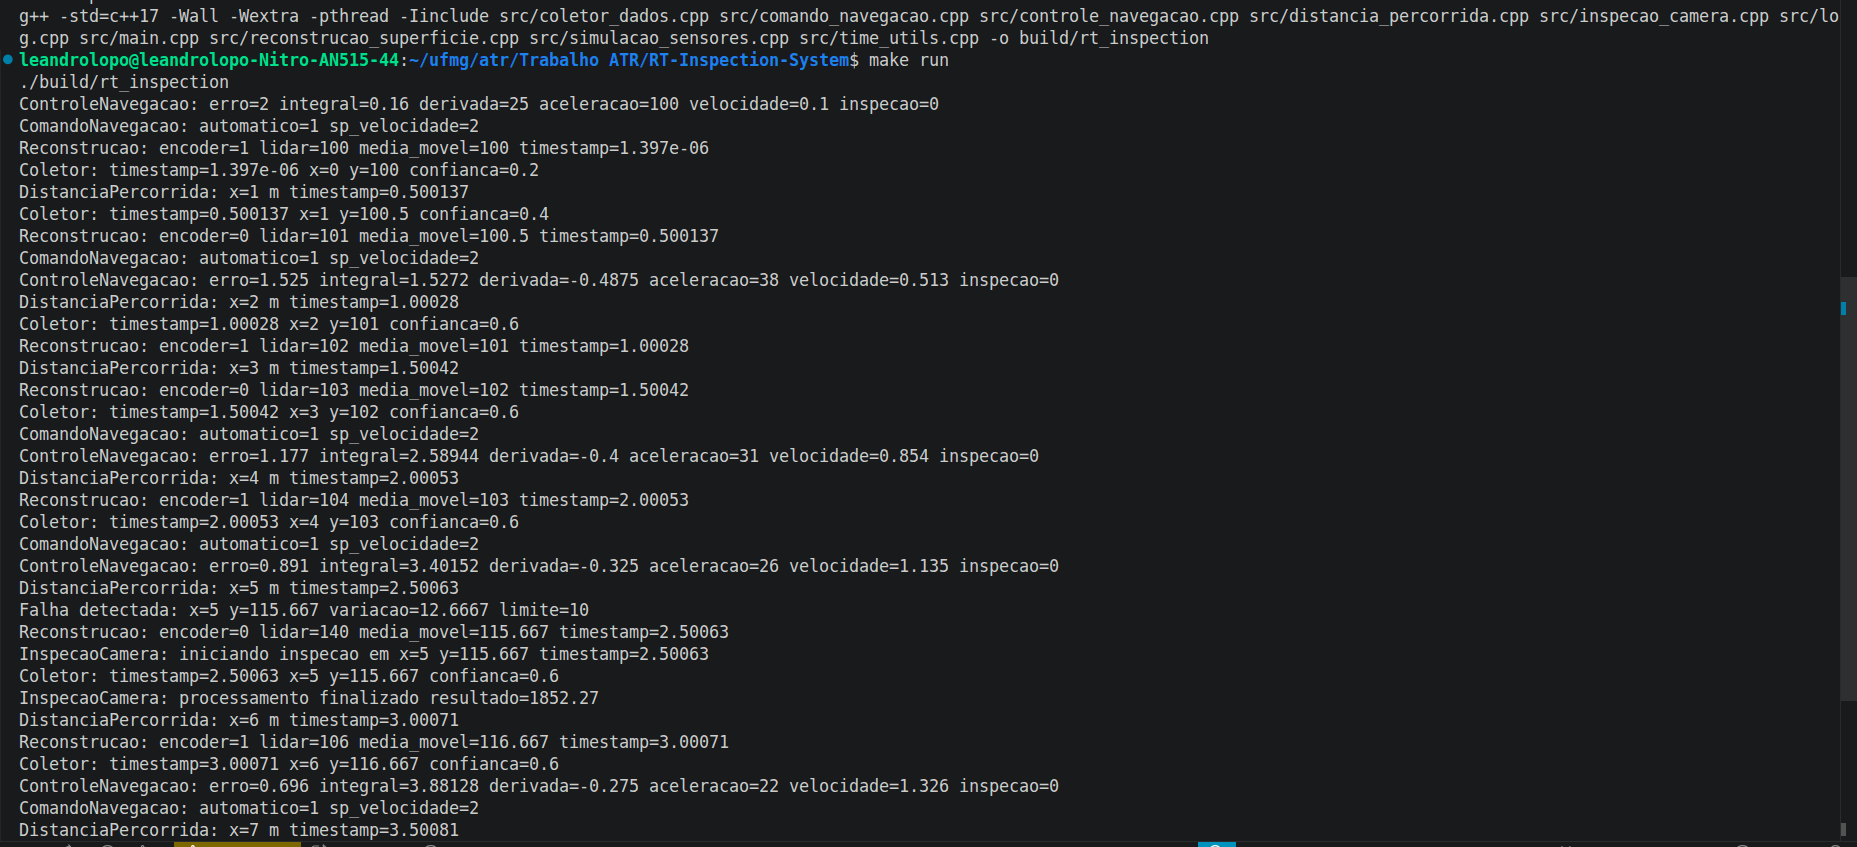
\includegraphics[width=\textwidth,height=0.42\textheight,keepaspectratio]{figuras/testes/terminal_completo.png}
        \caption{Print do terminal com a execução completa do sistema.}
        \label{fig:terminal-completo}
    \end{figure}

    \subsection{Teste 1: Troca de Dados entre Simulação e Reconstrução}

    O primeiro teste verificou se a tarefa \texttt{SimulacaoSensores} produz leituras de sensores e se a tarefa \texttt{ReconstrucaoSuperficie} consome essas leituras corretamente. O resultado esperado é a impressão de leituras com o valor filtrado por média móvel. A saída observada é mostrada na Figura~\ref{fig:teste-4-1-terminal}.

    \FiguraTesteTerminal
    {figuras/testes/teste_4_1_terminal.png}
    {Print do terminal do Teste 4.1: troca de dados entre simulação e reconstrução.}
    {fig:teste-4-1-terminal}

    Esse teste valida o funcionamento do \texttt{SensorBuffer}, do mutex associado e da variável de condição usada para acordar a reconstrução.

    \subsection{Teste 2: Cálculo de Distância Percorrida}

    O segundo teste verificou se o encoder é processado pela tarefa \texttt{DistanciaPercorrida}. Como o encoder simulado troca de estado a cada leitura, a posição horizontal é incrementada quando ocorre uma mudança. A saída observada é mostrada na Figura~\ref{fig:teste-4-2-terminal}.

    \FiguraTesteTerminal
    {figuras/testes/teste_4_2_terminal.png}
    {Print do terminal do Teste 4.2: cálculo da distância percorrida a partir do encoder.}
    {fig:teste-4-2-terminal}

    Esse teste valida o \texttt{EncoderBuffer}, o uso de \texttt{SharedRobotState} para manter a posição global e o \texttt{PositionBuffer} usado para entregar posições à reconstrução na mesma ordem das leituras.

    \subsection{Teste 3: Coletor de Dados e Arquivo CSV}

    O terceiro teste verificou se a reconstrução gera pontos de superfície e se o coletor consome esses pontos, calcula confiança e grava o arquivo \texttt{surface\_points.csv}. A saída observada é mostrada na Figura~\ref{fig:teste-4-3-terminal}.

    \FiguraTesteTerminal
    {figuras/testes/teste_4_3_terminal.png}
    {Print do terminal do Teste 4.3: verificação do arquivo CSV gerado pelo coletor de dados.}
    {fig:teste-4-3-terminal}

    Esse teste valida o \texttt{SurfaceBuffer}, o cálculo online de confiança e a gravação dos dados em disco.

    \subsection{Teste 4: Detecção de Falha e Acionamento da Câmera}

    O quarto teste inseriu uma anomalia no LIDAR simulado, configurando uma leitura com valor mais alto que o padrão. A reconstrução compara a média móvel atual com a média anterior e sinaliza falha quando a variação passa do limite configurado. A saída observada é mostrada na Figura~\ref{fig:teste-4-4-terminal}.

    \FiguraTesteTerminal
    {figuras/testes/teste_4_4_terminal.png}
    {Print do terminal do Teste 4.4: detecção de falha e acionamento da inspeção por câmera.}
    {fig:teste-4-4-terminal}

    Esse teste valida o \texttt{CameraEvent}, a sincronização por evento e o processamento pesado da tarefa de câmera. A câmera executa um laço com funções matemáticas, usando CPU de fato, e não apenas uma chamada de \texttt{sleep}.

    \subsection{Teste 5: Comando e Controle de Navegação}

    O quinto teste verificou se as tarefas cíclicas de comando e controle executam em paralelo com as demais tarefas. O comando fixa o modo automático e o setpoint de velocidade, enquanto o controle PID calcula a aceleração a partir do erro de velocidade. A saída observada é mostrada na Figura~\ref{fig:teste-4-5-terminal}.

    \FiguraTesteTerminal
    {figuras/testes/teste_4_5_terminal.png}
    {Print do terminal do Teste 4.5: execução das tarefas de comando e controle de navegação.}
    {fig:teste-4-5-terminal}

    Esse teste valida o uso de \texttt{SharedCommand}, \texttt{SharedRobotState}, \texttt{SharedActuatorData} e \texttt{SharedSystemControl}. Também mostra que as tarefas cíclicas encerram corretamente após a finalização das tarefas de simulação, reconstrução, coleta e câmera.

    \subsection{Análise dos Testes}

    Durante os testes, as threads finalizaram corretamente, sem bloqueio observado. Os buffers possuem flags de finalização para evitar que consumidores fiquem bloqueados indefinidamente. As impressões no terminal são protegidas por um mutex global de log, evitando mensagens misturadas. O \texttt{PositionBuffer} remove a dependência do escalonamento entre distância e reconstrução, pois a reconstrução passa a consumir a posição calculada na mesma ordem das leituras de sensor.

    \section{Conclusão}

    Nesta etapa foi implementado o núcleo embarcado do sistema de inspeção automática de túneis. As principais tarefas foram modeladas como threads C++ dentro de um único processo. Foram implementados buffers sincronizados para comunicação entre tarefas, estados compartilhados protegidos por mutex, reconstrução do perfil do teto por média móvel, cálculo de distância percorrida pelo encoder, envio ordenado de posição para reconstrução, controle PID simples, detecção de falha por variação brusca e acionamento de inspeção por câmera via evento.

    Os testes preliminares indicam que a arquitetura implementada consegue trocar dados entre tarefas sem condições de corrida aparentes, sem bloqueios observados e com finalização controlada das threads. O sistema também gera um arquivo CSV com os pontos reconstruídos, permitindo verificar o perfil estimado do teto.

    Como próximos passos para a Etapa 2, devem ser implementadas as interfaces gráficas de simulação e operação remota, a comunicação entre processos via MQTT, a integração com um broker publisher/subscriber e uma análise mais detalhada de tempo de resposta e escalonabilidade das tarefas cíclicas.

    \end{document}
